\documentclass{article}

\usepackage{amsmath}
\usepackage{amssymb}
\usepackage{algorithm}
\usepackage[noend]{algpseudocode}		% for algorithms in pseudo code. Usage: \begin{algorithmic}
\usepackage{subcaption}
\usepackage{tikz}
\usetikzlibrary{decorations.pathmorphing}
\usetikzlibrary{decorations.markings}
\usetikzlibrary{calc}
\colorlet{burgundy}{red!75!black}

\newcommand{\vecl}{\overrightarrow} % long vector for multiple characters
\newcommand{\len}[1]{\left\lVert #1 \right\rVert}
\newcommand{\inta}{\operatorname{int}} % interior angle
\newcommand{\exta}{\operatorname{ext}} % exterior angle

\title{Determining the Convexity of any Polygon}
\author{Abraham Murciano}

\begin{document}
\maketitle

\section{Abstract}

This paper presents and proves the correctness of an algorithm which determines if a sequence of points in three-dimensional space forms a convex polygon or not. We will discuss simple convex and concave polygons as well as complex (self intersecting) polygons, and ultimately even non-planar polygons.

\section{Definitions}

\begin{description}
	\item[Turn between vectors]
		The turn between two three-dimensional vectors \(\vec{u}\) and \(\vec{v}\), which we shall denote henceforth as \(T(\vec{u}, \vec{v}) \in [0, \pi]\), is defined as follows.
		\begin{equation*}
			T(\vec{u}, \vec{v}) = \arccos \left( \frac{\vec{u} \cdot \vec{v}} {\len{\vec{u}} \cdot \len{\vec{v}}} \right)
		\end{equation*}
		For any two vectors there are two angles between them, and the function \(T\) always gives us the smaller of the two.

	\item[Polygon]
		A polygon is a sequence of at least three points (also called vertices) in three-dimensional space where each point is connected to the next by a straight line segment called an edge. There is also an edge between the last and first points. The edges form a closed path.

		Most definitions of a polygon are in fact what we will refer to as a simple polygon, but since we are interested in processing any given sequence of points, and to simplify our language in this paper, we shall extend our definition of a polygon to include any such sequences.

	\item[Planar polygon]
		A planar polygon is a polygon whose vertices all share a common plane.

	\item[Non-planar polygon]
		A non-planar polygon is simply a polygon which is not planar.

	\item[Simple polygon]
		A simple polygon is a planar polygon whose bounding edges do not intersect with one another. That is, their edges to not touch each other except for each edge touching exactly one edge at each of its end points.

	\item[Convex polygon]
		A polygon is convex if it is simple and all its interior angles are less than \(\pi\) radians.

	\item[Concave polygon]
		A polygon is concave if it is simple and not convex. That is, if it has an interior angle greater than \(\pi\) radians.

	\item[Complex polygon]
		A polygon is complex if it is planar, but not simple. That is, if its edges intersect with each other.

	\item[Turn of a polygon at a vertex]
		If \(A\), \(B\), and \(C\) are three adjacent vertices of a polygon \(P\) such that \(B\) is in between \(A\) and \(C\), the turn of the polygon at the point \(B\) is \(T_P(B) = T(\vecl{AB}, \vecl{BC})\).

		Note, for polygons for which the term `exterior angle' is defined, the turn at a vertex is equal to the absolute value of the exterior angle at that vertex.

	\item[Total turn of a polygon]
		The total turn of a polygon \(P\), is the sum of the turns of all its vertices. We shall use the following shorthand notation to denote this.
		\begin{equation*}
			\sum T_P = \sum_{v \in P} T_P(v)
		\end{equation*}
\end{description}

\begin{figure}[htbp]
	\centering
	\begin{subfigure}{0.25\textwidth}
		\centering
		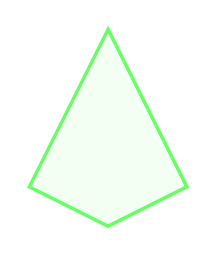
\begin{tikzpicture}
			\filldraw[color=green!60, fill=green!5, very thick] (0, 0) -- (1, -0.5) -- (2, 0) -- (1, 2) -- cycle;
		\end{tikzpicture}
		\caption{Convex}
	\end{subfigure}%
	\begin{subfigure}{0.25\textwidth}
		\centering
		
\begin{tikzpicture}
			\filldraw[color=orange!60, fill=orange!5, very thick] (0, 0) -- (1, 0.5) -- (2, 0) -- (1, 2.5) -- cycle;
		\end{tikzpicture}
		\caption{Concave}
	\end{subfigure}%
	\begin{subfigure}{0.25\textwidth}
		\centering
		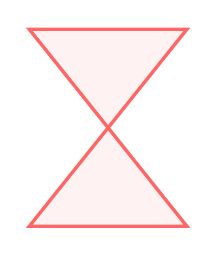
\begin{tikzpicture}
			\filldraw[color=red!60, fill=red!5, very thick] (0, 0) -- (2, 2.5) -- (0, 2.5) -- (2, 0) -- cycle;
		\end{tikzpicture}
		\caption{Complex}
	\end{subfigure}%
	\caption{Examples of different types of polygons.}
	\label{}
\end{figure}

\section{The Algorithm}

We will begin by explaining how the algorithm works, then presenting the algorithm at the end of this section.

\subsection{Input}

The algorithm accepts a sequence of points \(P\) in three-dimensional space. The points represent a polygon formed by constructing an edge between all adjacent vertices in the sequence and an additional edge between the first and last vertices.

\subsection{Output}

The algorithm returns True if the input forms a convex polygon, and False if they form any other type of polygon.

\subsection{Processing} \label{processing}

First, if at least three consecutive points lie consecutively on a single line, the middle points may be removed as they contribute nothing to the polygon and are thus meaningless. The check necessary to do this is simple enough and has been omitted for conciseness. From now on we may assume that any such cases are corrected before any further processing is performed.

The algorithm then boils down to a single check. A sequence of vertices forms a simple convex polygon if and only if the sum of the turns is equal to \(2\pi\). Formally, the algorithm checks if the following equation holds true.

\begin{equation*}
	\sum T_P = 2\pi
\end{equation*}

\subsection{Pseudo Code}

The function \textsc{IsConvex} takes as input a sequence of points \(P\) and returns whether or not the points form a convex polygon.

\begin{algorithm}[htbp]
	\begin{algorithmic}
		\Function{IsConvex}{$P$}
		\State Remove meaningless vertices from \(P\)
		\If{\(|P| < 3\)}
		\Return False
		\EndIf
		\State \(\Sigma := 0\) \Comment{The running sum of the turn.}
		\For{\(i\) from 0 to \(|P| - 1\)}
		\State \(A := P_{i-1 \mod |P|}\) \Comment{The previous point.}
		\State \(B := P_{i}\) \Comment{The current point.}
		\State \(C := P_{i+1 \mod |P|}\) \Comment{The next point.}
		\State \(\Sigma := \Sigma + T(\vecl{AB}, \vecl{BC})\) \Comment{Add the turn at point \(B\).}
		\EndFor
		\State\Return \(\Sigma = 2\pi\)
		\EndFunction
	\end{algorithmic}
\end{algorithm}

\section{Proof of Correctness}

\subsection{Claim}

A sequence of vertices \(P\) forms a convex polygon if and only if the total turn \(\sum T_P\) is equal to \(2\pi\).

In order to prove our claim, we must prove all of the following cases.
\begin{enumerate}
	\item If a polygon is convex then the total turn is equal to \(2\pi\).
	\item If a polygon is concave then the total turn is greater than \(2\pi\).
	\item If a polygon is complex then the total turn is greater than \(2\pi\).
	\item If a polygon is non-planar, then the total turn is greater than \(2\pi\).
\end{enumerate}

\subsection{Proof}

\subsubsection{Convex Polygons Have a Total Turn of Precisely \(2\pi\)}

It is known that the exterior angles of a simple polygon sum to precisely \(2\pi\). An exterior angle is defined as \(\pi\) minus the interior angle. However since by definition of a convex polygon all its interior angles are less than \(\pi\), the exterior angles must be positive.

Therefore for a convex polygon \(P\), we have
\begin{equation*}
	\sum T_P = \sum_{v \in P} T_P(v) = \sum_{v \in P} | \exta(v) | = \sum_{v \in P} \exta (v) = 2\pi
\end{equation*}
where \(\exta (v)\) is the exterior angle at vertex \(v\).

\subsubsection{The Total Turn of a Concave Polygon Exceeds \(2\pi\)}

A concave polygon must have at least one negative exterior angle. This is because it must have, by definition, at least one interior angle greater than \(\pi\) radians. Since \(\exta(v) = \pi - \inta(v)\), where \(\inta(v)\) is the interior angle, \(\exta(v)\) must be negative for some vertex \(v\).

Therefore for a concave polygon \(P\), we have the following inequality.
\begin{equation*}
	\sum T_P = \sum_{v \in P} T_P(v) = \sum_{v \in P} | \exta(v) | > \sum_{v \in P} \exta(v) = 2\pi
\end{equation*}

\subsubsection{A Complex polygon's Total Turn Exceeds \(2\pi\)}

The first thing to do is to disqualify any polygon with overlapping colinear (not necessarily consecutive) edges. If a walk through the edges would demonstrate that these edges are walked through in the same direction twice that means that a total turn of at least \(2\pi\) has already been made between the two edges, yet the traversal has not yet concluded. Otherwise, if the edges are walked over in opposite directions, that would require a total turn of at least \(\pi\) to turn around at each end of these edges. If that is all the turns that there are, then this sequence of points has only two significant points and does not form a polygon. As explained in section \ref{processing}, we may assume this is not the case. Now that we've gotten that out of the way, we may proceed with the assumption that no edges overlap.

For any complex polygon \(P\), we are able to find a sequence of consecutive vertices of \(P\) which when appended to an intersection point of \(P\) forms a simple polygon in the following way.

We choose any arbitrary point on the polygon's bounding path. Then from that point we trace the bounding path, marking any intersection points we encounter. Once we arrive at an intersection point which we've previously encountered, we stop. Let this intersection point be called \(I\).

The closed path which we traced from the first encounter with \(I\) to our second encounter with \(I\) is a simple polygon (see figure \ref{simple-polygon-extraction}).

\begin{figure}[htbp]
	\centering
	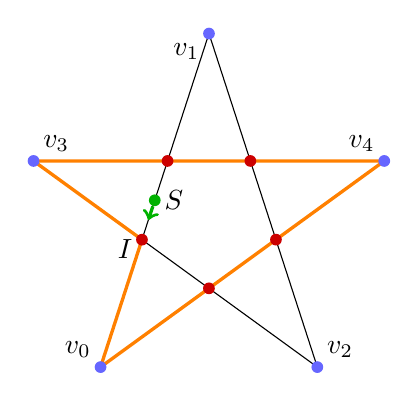
\begin{tikzpicture}
		[point/.style={circle, inner sep=1.5pt},
			vertex/.style={point, fill=blue!60!white},
			intersection/.style={point, fill=red!80!black}]
		% define pentagram's vertices
		\coordinate (v0) at (0, 0);
		\coordinate (v1) at (1.377, 4.236);
		\coordinate (v2) at (2.753, 0);
		\coordinate (v3) at (-0.851, 2.618);
		\coordinate (v4) at (3.603, 2.618);
		% define intersection points
		\coordinate (i0) at (intersection of v1--v2 and v3--v4);
		\coordinate (i1) at (intersection of v2--v3 and v4--v0);
		\coordinate (i2) at (intersection of v3--v4 and v0--v1);
		\coordinate (i3) at (intersection of v4--v0 and v1--v2);
		\coordinate (i4) at (intersection of v0--v1 and v2--v3);
		% draw the pentagram
		\draw (v0) to (v1) to (v2) to (v3) to (v4) to cycle;
		% draw extracted simple polygon
		\draw[very thick, color=orange] (i4) to (v0) to (v4) to (v3) to cycle;
		% label the vertices
		\node[anchor=south east] at (v0) {\(v_0\)};
		\node[anchor=north east] at (v1) {\(v_1\)};
		\node[anchor=south west] at (v2) {\(v_2\)};
		\node[anchor=south west] at (v3) {\(v_3\)};
		\node[anchor=south east] at (v4) {\(v_4\)};
		% mark the vertices
		\node[vertex] at (v0) {};
		\node[vertex] at (v1) {};
		\node[vertex] at (v2) {};
		\node[vertex] at (v3) {};
		\node[vertex] at (v4) {};
		% mark the intersections
		\node[intersection] at (i0) {};
		\node[intersection] at (i1) {};
		\node[intersection] at (i2) {};
		\node[intersection] at (i3) {};
		\node[intersection] at (i4) {} node[anchor=30] at (i4) {\(I\)};
		% define and label starting point
		\node[point, fill=green!70!black] (S) at (intersection of v3--i3 and v0--v1) {} node[anchor=west] at (S) {\(S\)};
		\draw[->, very thick, green!70!black] (S) to ($(S)!0.5!(i4)$);
	\end{tikzpicture}
	\caption{Extracting a simple polygon from a complex one. This complex polygon is a pentagram with vertices \(v_0\) through \(v_4\). \(S\) is the arbitrarily chosen starting point. The orange arrowhead marks the bounding edges of a simple polygon \(E = (v_0, v_4, v_3, I)\) embedded in the complex pentagram. \(I\) is the first (and necessarily the only) intersection point of the pentagram which we encountered twice.}
	\label{simple-polygon-extraction}
\end{figure}

The embedded polygon \(E\) found with this procedure must be simple since we stop our trace at the first intersection point we encounter twice, and we never retrace our steps. Thus all of \(P\)'s intersection points are touched only once by \(E\), except for point \(I\) which is the start and end point, so is not an intersection point of \(E\) either.

Let \(\alpha \in (-\pi, \pi)\) be the exterior angle of \(E\) at vertex \(I\). Since \(E\) is a simple polygon it can't have exterior angles of \(\pm\pi\), else the bounding edges would go back on themselves contradicting \(E\)'s simplicity.

Suppose now we were to `walk' a cycle through the edges of \(P\) starting at the midpoint of the line segment formed by \(I\) and one of the two vertices adjacent to \(I\) which is common to both \(P\) and \(E\) (either \(v_0\) or \(v_3\) in figure \ref{simple-polygon-extraction}). Suppose we start walking in the direction away from \(I\) and are only allowed to walk forward and turn.

The first time we reach \(I\), we will have already turned all the turns of \(E\) but one --- \(T_E(I)\), which is equal to \(|\alpha|\). We immediately pass \(I\) and enter a section of the path which is no longer part of \(E\). Let us analyze the current position.

Since \(I\) is an intersection point of \(P\), we will in future be forced to encounter it again before arriving finally at the start. However, since we've just passed \(I\), it is positioned a small distance directly behind us. This means that in order to reach it in future, our path must force us to make some turns which sum to at least \(\pi\) radians.

This now allows us to formulate our first inequality.
\begin{equation}
	\sum T_P \geq \sum T_E - |\alpha| + \pi \label{ineq-1}
\end{equation}

Since we know that \(\sum T_E \geq 2\pi\) due to the simplicity of \(E\), and that \(|\alpha| \in [0, \pi)\), we can from inequality \ref{ineq-1} come to the following conclusion.
\begin{equation}
	\sum T_P \geq 3\pi - |\alpha| > 2\pi
\end{equation}

\end{document}